\chapter{สถาปัตยกรรมโมเดลการเรียนรู้เชิงลึกฟิวชันภาพถ่ายและเซนเซอร์}
\label{ch:multimodal_deep_learning}

\section{บทนำและแนวคิดการผสานข้อมูลหลากมิติ}

การวิเคราะห์คุณสมบัติดินให้มีความแม่นยำระดับห้องปฏิบัติการบนอุปกรณ์พกพา จำเป็นต้องก้าวข้ามข้อจำกัดของโมเดลการเรียนรู้แบบเดี่ยว (Single-modality Learning) ในระบบที่พัฒนาขึ้นนี้ คณะผู้วิจัยได้ออกแบบสถาปัตยกรรมโมเดลโครงข่ายประสาทเทียมเชิงลึกแบบฟิวชันหลากมิติ (Multimodal Deep Fusion Network) ซึ่งทำหน้าที่ผสานเวกเตอร์คุณลักษณะเชิงแสงที่ได้จากภาพถ่าย 9 มิติ เข้ากับเวกเตอร์คุณลักษณะทางกายภาพที่ตรวจวัดได้จากหัววัด 7-in-1 อีก 7 มิติ เกิดเป็นเวกเตอร์ข้อมูลนำเข้ารวม 16 มิติที่มีความสมบูรณ์สูงสุด

\section{เวกเตอร์ข้อมูลนำเข้าและกระบวนการปรับมาตรฐาน}

เวกเตอร์ข้อมูลนำเข้ารวม ($\mathbf{x} \in \mathbb{R}^{16}$) ประกอบด้วยตัวแปรคุณลักษณะสองกลุ่มหลักดังต่อไปนี้

\begin{equation}
\mathbf{x} = \begin{bmatrix} \mathbf{x}_{\text{vision}} \\ \mathbf{x}_{\text{sensor}} \end{bmatrix} \in \mathbb{R}^{16}
\end{equation}

โดยที่เวกเตอร์ฝั่งคอมพิวเตอร์วิทัศน์ ($\mathbf{x}_{\text{vision}} \in \mathbb{R}^9$) ประกอบด้วยค่าพิกัดสีที่ผ่านการปรับมาตรฐาน

\begin{equation}
\mathbf{x}_{\text{vision}} = \left[ R_{\text{norm}}, \, G_{\text{norm}}, \, B_{\text{norm}}, \, \frac{H}{360}, \, S, \, V, \, \frac{L^*}{100}, \, \frac{a^* + 128}{255}, \, \frac{b^* + 128}{255} \right]^T
\end{equation}

และเวกเตอร์ฝั่งเซนเซอร์หัววัดภาคสนาม ($\mathbf{x}_{\text{sensor}} \in \mathbb{R}^7$) สกัดจากหัววัดอิเล็กโทรด 7-in-1 ดังแสดงในภาพที่ \ref{fig:soil_probe_hardware}

\begin{figure}[H]
\centering
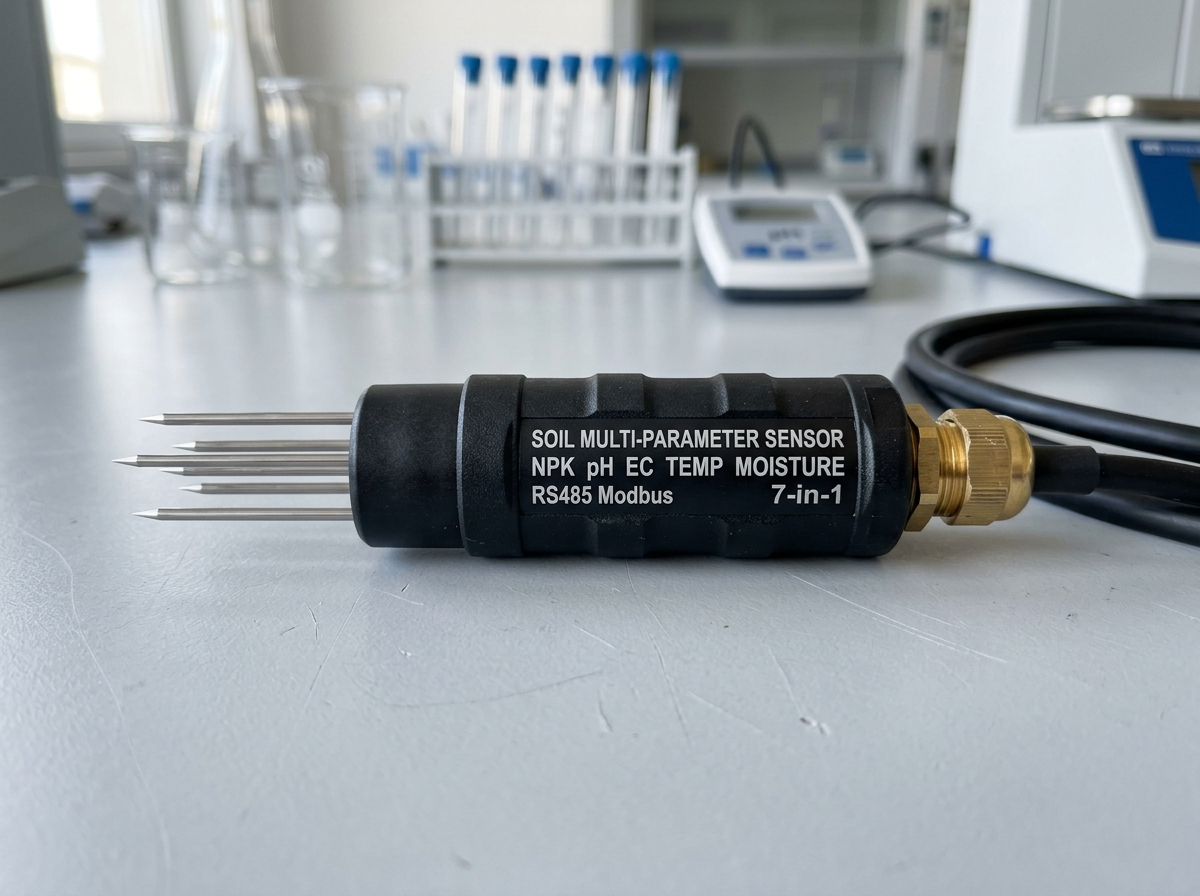
\includegraphics[width=0.65\textwidth]{figures/soil_probe_7in1.jpg}
\caption{หัววัดดินอิเล็กโทรดโลหะ 7-in-1 สำหรับเก็บรวบรวมตัวแปรทางกายภาพและเคมี 7 มิติ}
\label{fig:soil_probe_hardware}
\end{figure}

\begin{equation}
\mathbf{x}_{\text{sensor}} = \left[ 
\frac{\text{Moisture}}{100}, \, 
\frac{\text{Temp} + 10}{60}, \, 
\frac{\text{EC}}{5000}, \, 
\frac{\text{pH}}{14}, \, 
\frac{\text{N}_{\text{sensor}}}{200}, \, 
\frac{\text{P}_{\text{sensor}}}{100}, \, 
\frac{\text{K}_{\text{sensor}}}{300} 
\right]^T
\end{equation}

\section{สถาปัตยกรรมโครงข่ายประสาทเทียมและการไหลของสัญญาณ}

โครงสร้างเครือข่ายได้รับการปรับแต่งให้มีขนาดกะทัดรัด (Edge-optimized Deep Architecture) เพื่อให้สามารถประมวลผลบนหน่วยประมวลผลของสมาร์ทโฟนได้โดยตรง โดยมีจำนวนพารามิเตอร์รวมไม่เกิน 500 พารามิเตอร์ จึงกินพลังงานต่ำมากและทำงานได้แบบ Zero-Latency

\begin{figure}[H]
\centering
\begin{tikzpicture}[
    scale=0.85, every node/.style={transform shape},
    node distance=1.6cm,
    layer/.style={rectangle, draw=rbruNavy, fill=rbruNavy!10, rounded corners, minimum height=0.9cm, minimum width=2.2cm, font=\bfseries\small, align=center},
    inputnode/.style={circle, draw=rbruBlue, fill=rbruBlue!15, minimum size=0.6cm, inner sep=0pt},
    hiddennode/.style={circle, draw=rbruTeal, fill=rbruTeal!20, minimum size=0.6cm, inner sep=0pt},
    outputnode/.style={circle, draw=rbruOrange, fill=rbruOrange!25, minimum size=0.65cm, inner sep=0pt},
    arrow/.style={-{Stealth[length=2.5mm]}, thick, draw=rbruSlate}
]

% Input Layers
\node[layer, fill=cyan!15] (visin) at (0, 3) {Vision Inputs\\(9 Features)};
\node[layer, fill=green!15] (sensin) at (0, -1) {Sensor Inputs\\(7 Features)};

% Concatenation
\node[layer, fill=rbruGold!25] (concat) at (4, 1) {Feature Fusion Layer\\$\mathbf{x} \in \mathbb{R}^{16}$};

% Hidden Layer 1
\node[layer, fill=rbruTeal!25] (h1) at (8, 1) {Dense Layer 1\\(12 Neurons)\\LeakyReLU ($\alpha=0.1$)};

% Output Heads
\node[layer, fill=rbruOrange!20] (out_som) at (13, 3) {SOM Head\\(\% อินทรียวัตถุ)};
\node[layer, fill=rbruOrange!20] (out_ph) at (13, 1.8) {Optical pH Head\\(ความเป็นกรดด่าง)};
\node[layer, fill=rbruOrange!20] (out_n) at (13, 0.6) {Predicted N Head\\(ไนโตรเจน mg/kg)};
\node[layer, fill=rbruOrange!20] (out_p) at (13, -0.6) {Predicted P Head\\(ฟอสฟอรัส mg/kg)};
\node[layer, fill=rbruOrange!20] (out_k) at (13, -1.8) {Predicted K Head\\(โพแทสเซียม mg/kg)};

% Connectors
\draw[arrow] (visin.east) -- (concat.west);
\draw[arrow] (sensin.east) -- (concat.west);
\draw[arrow] (concat.east) -- (h1.west);
\draw[arrow] (h1.east) -- (out_som.west);
\draw[arrow] (h1.east) -- (out_ph.west);
\draw[arrow] (h1.east) -- (out_n.west);
\draw[arrow] (h1.east) -- (out_p.west);
\draw[arrow] (h1.east) -- (out_k.west);

\end{tikzpicture}
\caption{แผนภาพสถาปัตยกรรมโครงข่ายประสาทเทียมฟิวชัน 16 มิติและการกระจายสู่ 5 เอาต์พุต}
\label{fig:multimodal_nn_arch}
\end{figure}

สมการการแปลงสถานะในชั้นซ่อนเร้นชั้นที่ 1 นิยามโดย

\begin{equation}
\mathbf{h}_1 = \text{LeakyReLU}\left( \mathbf{W}_1 \mathbf{x} + \mathbf{b}_1, \, \alpha = 0.1 \right)
\end{equation}

โดยที่ $\mathbf{W}_1 \in \mathbb{R}^{12 \times 16}$ และ $\mathbf{b}_1 \in \mathbb{R}^{12}$ จากนั้นสัญญาณจะถูกส่งผ่านเวกเตอร์น้ำหนักของแต่ละหัวเป้าหมายเพื่อทำนายค่าคุณสมบัติดินออกมา

\begin{align}
\widehat{\text{SOM}} &= \sigma\left( \mathbf{w}_{\text{SOM}}^T \mathbf{h}_1 + b_{\text{SOM}} \right) \times 10.0 \\
\widehat{\text{pH}}_{\text{opt}} &= 3.5 + 6.0 \times \sigma\left( \mathbf{w}_{\text{pH}}^T \mathbf{h}_1 + b_{\text{pH}} \right)
\end{align}

\section{การตรวจจับความผิดปกติและการตรวจสอบความสอดคล้อง}

หัวใจสำคัญของการประยุกต์ใช้ปัญญาประดิษฐ์ในระบบเซนเซอร์เกษตรแม่นยำ คือการสร้างความเชื่อถือได้ของข้อมูล (Sensor Fault Tolerance) ระบบจึงมีกลไกตรวจสอบค่าผลต่างสัมบูรณ์ของความเป็นกรดด่าง ($\Delta\text{pH}$) ระหว่างหัววัดไฟฟ้าและคอมพิวเตอร์วิทัศน์

\begin{equation}
\Delta\text{pH} = \left| \text{pH}_{\text{sensor}} - \widehat{\text{pH}}_{\text{opt}} \right|
\end{equation}

ระบบประเมินสถานะความสอดคล้องออกเป็น 3 ระดับ ดังนี้
\begin{enumerate}[label=\textbf{\arabic*.}]
\item \textbf{ความสอดคล้องสูงมาก ($\Delta\text{pH} \le 0.50$)} ข้อมูลทั้งสองมิติสอดรับกันอย่างสมบูรณ์แบบ โมเดลให้ระดับความเชื่อมั่นสูงสุด (High Confidence)
\item \textbf{ความสอดคล้องปานกลาง ($0.50 < \Delta\text{pH} \le 1.00$)} เริ่มมีความแตกต่างเล็กน้อย ซึ่งอาจเกิดจากความไม่สม่ำเสมอของเนื้อดินหรือความชื้นเฉพาะจุด
\item \textbf{พบความผิดปกติของข้อมูล ($\Delta\text{pH} > 1.00$)} สัญญาณแจ้งเตือนความผิดปกติ (Anomaly Warning) จะปรากฏบนหน้าจอ เพื่อให้ผู้ใช้ตรวจสอบการปนเปื้อนที่ผิวสัมผัสหัววัด หรือแสงรบกวนในภาพถ่าย
\end{enumerate}

\begin{figure}[H]
\centering
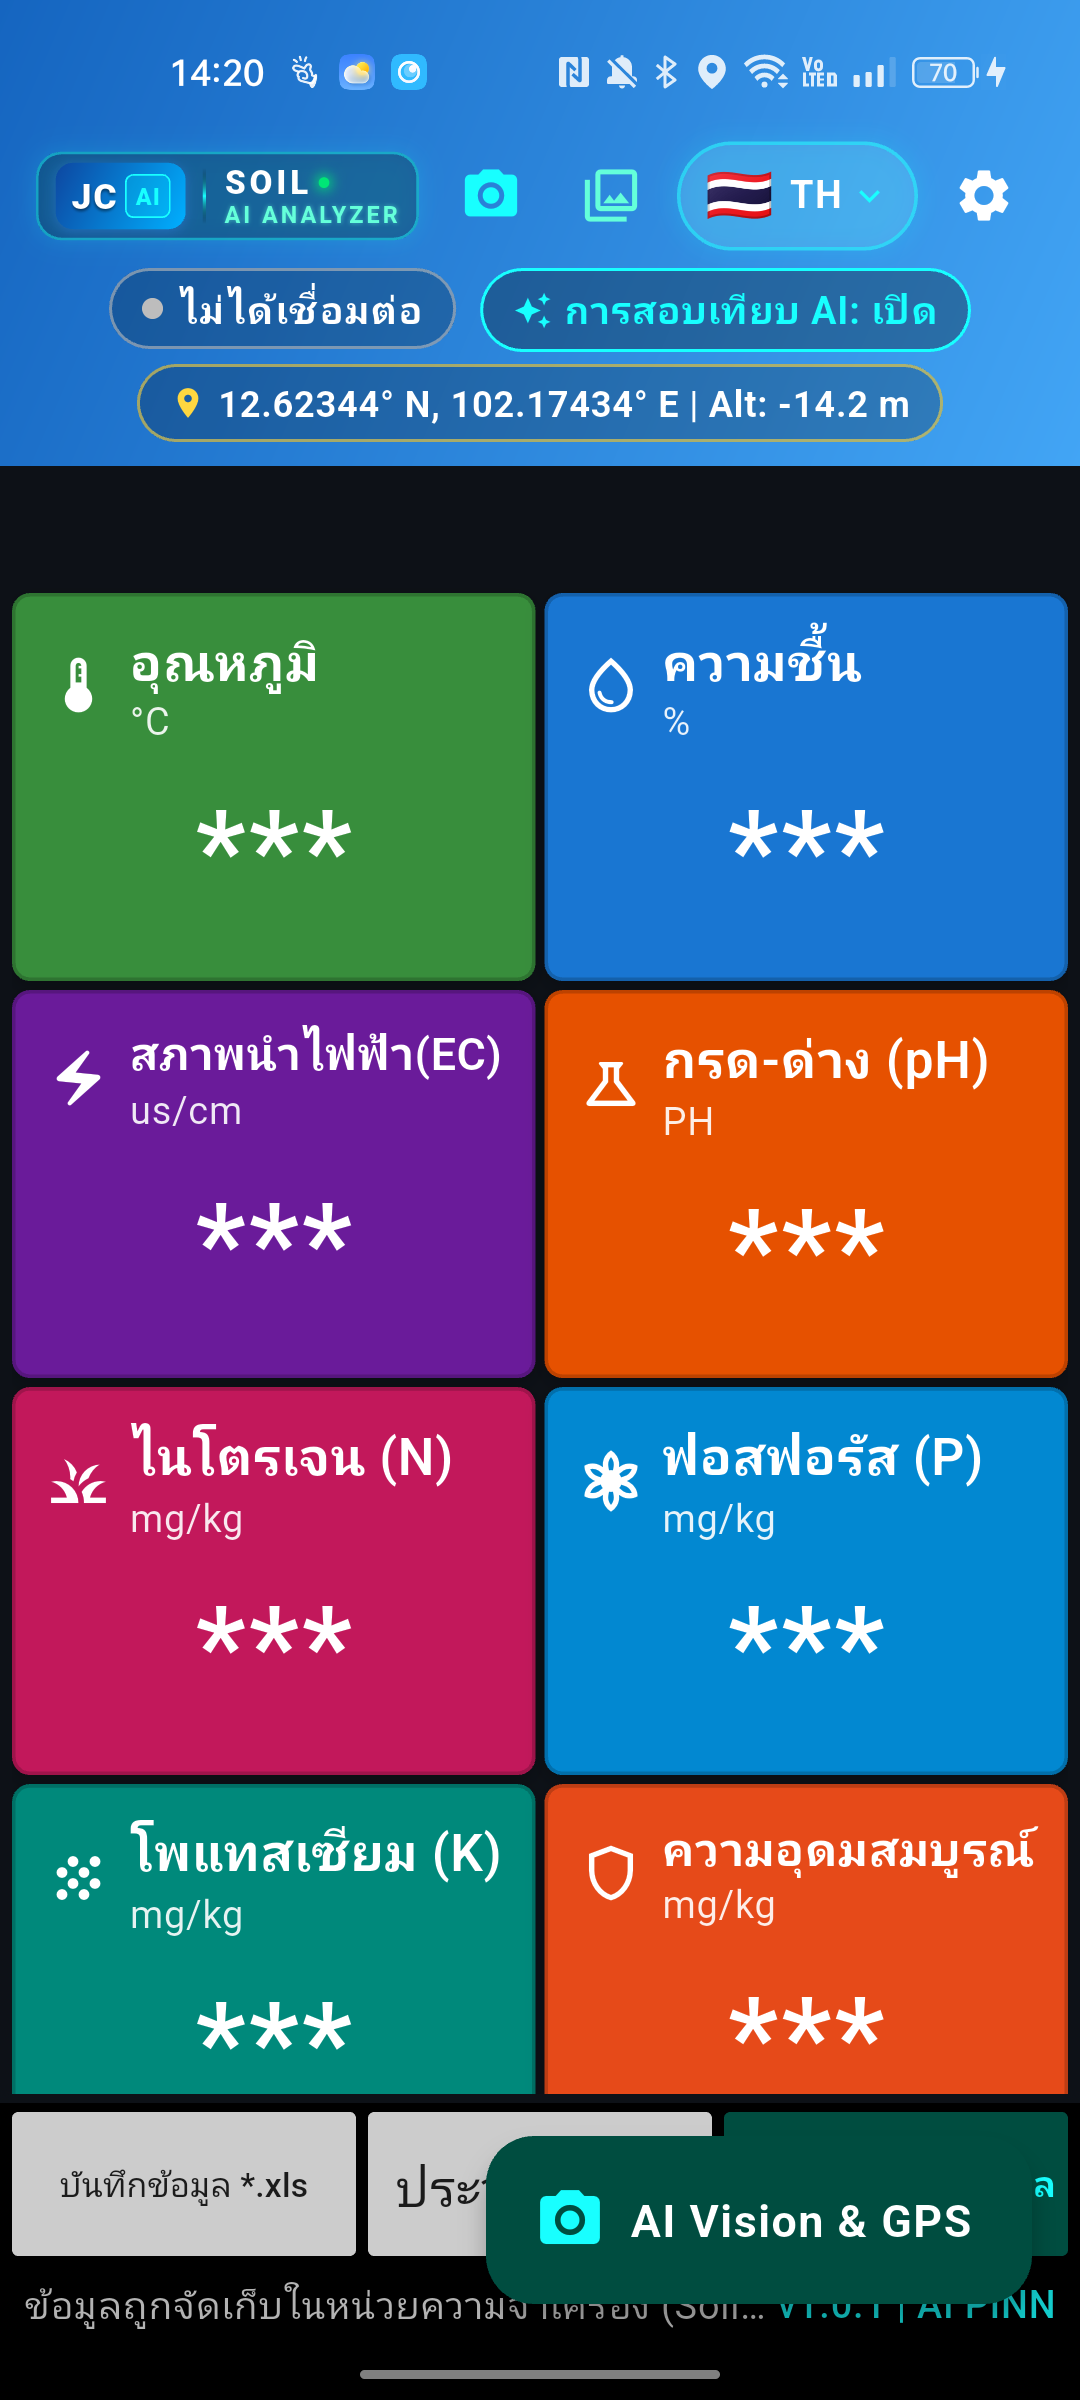
\includegraphics[width=0.75\textwidth]{figures/app_dashboard_live.png}
\caption{แดชบอร์ดแสดงผลการวิเคราะห์เปรียบเทียบระหว่างค่าภาพถ่ายและค่าเซนเซอร์ภาคสนาม}
\label{fig:app_dashboard_live}
\end{figure}

ภาพที่ \ref{fig:app_dashboard_live} แสดงหน้าจอแดชบอร์ดหลักของแอปพลิเคชันที่นำเสนอการวิเคราะห์เปรียบเทียบแบบขนานระหว่างคุณลักษณะสี ปริมาณธาตุอาหาร N-P-K และดัชนีความสอดคล้อง $\Delta\text{pH}$ แบบเรียลไทม์
